\documentclass[conference,a4paper]{IEEEtran}
\IEEEoverridecommandlockouts
\usepackage[utf8]{inputenc}
\usepackage[T1]{fontenc}
\usepackage{amsmath,amssymb}
\usepackage{graphicx}
\usepackage{booktabs}
\usepackage{array}
\usepackage{xcolor}
\usepackage{tikz}
\usetikzlibrary{arrows.meta,positioning,fit,calc}
\usepackage{pgfplots}
\pgfplotsset{compat=1.18}
\usepackage{xurl}
\usepackage[hidelinks]{hyperref}
\usepackage{cite}

\definecolor{blockfill}{HTML}{EEF2F7}
\definecolor{blockline}{HTML}{44546A}
\definecolor{accentA}{HTML}{3B6FB6}
\definecolor{accentB}{HTML}{D98A2B}
\definecolor{accentC}{HTML}{6A9F58}

\newcommand{\code}[1]{\texttt{\small #1}}
% Straight double quotes around #1.
\newcommand{\q}[1]{\textquotedbl{}#1\textquotedbl{}}

\begin{document}

\title{On-device planning and stem-aware playback\\of DJ-style transitions in AutoMix,\\a native macOS music client}

\author{\IEEEauthorblockN{Claude Opus 5.5}
\IEEEauthorblockA{Anthropic, model \code{claude-opus-5-5}, with extended thinking at the xhigh effort level, in Claude Code\\
Technical report on AutoMix version 2 for the YouTube Music with AutoMix project, named Metrolist on the Mac.\\
It describes branch \code{claude/merge-2026-11-21} as of 22 November 2026 and replaces the report of 14 November 2026.}}

\maketitle

\begin{abstract}
AutoMix is the transition system of a native macOS client for YouTube Music. Instead of a fixed
cross-fade, it plans a transition for every pair of consecutive songs and performs it on a
two-deck audio engine, all on the listener's computer. This report describes the second version of
the system. The app analyses each song once for tempo, beats, bars, key, harmony, tone colour and
sections. A small neural beat tracker runs through Core ML and corrects one class of tempo error,
a pulse counted at two-thirds or three-halves of the real beat. A planner proposes and ranks four
kinds of transition. These are blends between phrases with the beats matched, hand-overs on shared
lyrics, dissolves between similar passages, and sample moves that bring the first song to the
speed and pitch at which the second song samples it. A logistic \q{sample gate}, trained on
reference mixes, decides whether an apparent sample is real. When two songs share no material, a
match that needs a speed change may change speed by at most 20\,\%, the range within which real DJs
make almost all their tempo changes. During playback the engine starts the two decks at an exact
time on the audio clock and keeps them in step with a phase lock. In the optional stem mode,
HT-Demucs separates the overlapping passages of both songs into vocals, drums, bass and the rest.
The outgoing vocals can then step aside and the basslines can swap instead of clashing. A learned
model orders the songs Autoplay adds. The report describes the design, the representation of a
transition and the testing method. The tests include approved reference pairs that must plan
byte-identically, parity tests against the original models, and audits over hundreds of song
pairs. The report closes with the measured results, the current limitations of the system, and
the limitations of research on automatic DJ mixing.
\end{abstract}

\begin{IEEEkeywords}
Automatic DJ mixing, music transitions, beat tracking, music source separation, time-stretching,
music information retrieval, Core ML, on-device machine learning.
\end{IEEEkeywords}

\section{Introduction}

Music streaming services have begun to join songs the way a DJ does. Spotify's Mix feature lets a
listener start from an automatic blend or a preset such as \q{Fade} or \q{Rise} and shape each
transition with volume, EQ and effect curves \cite{spotifymix}. Apple describes its AutoMix as
\q{Using AI to analyse audio features} to build transitions \q{with time stretching and beat
matching} \cite{applemix}. Neither service publishes how it chooses a transition or how it was
evaluated.

This report describes AutoMix, the transition system of an unofficial, open-source macOS client
for YouTube Music. The client follows the design of the Android client Metrolist
\cite{metrolist}. AutoMix differs from a plain cross-fade in four ways.
\begin{itemize}
\item \emph{A reason to mix.} The planner searches each pair of songs for a musical reason to join
them. It looks for phrase boundaries that line up, words both songs sing, passages that sound
alike, and samples one song takes from the other.
\item \emph{DJ practice.} The playing song makes large tempo and key changes \emph{before} the
overlap, the way a DJ adjusts the pitch fader before bringing in the next record. Both songs then
run beat for beat.
\item \emph{On the device.} The Mac analyses, separates and mixes the audio. Apart from fetching
the songs' audio and line-timed lyrics, the only network use is an optional title-and-artist query
to a sample database.
\item \emph{Explainable and editable.} A transition is data. An editor shows each transition with
the reason the planner chose it, and the listener can change it.
\end{itemize}

A report on 14 November 2026 described the first version. Since then the analysis has gained a
neural beat-error correction. The planner has gained a learned sample gate, tempo ramps and a limit
on speed changes between unrelated songs. The engine has gained stem separation, and the queue a
learned ordering model. Section~\ref{sec:background} introduces the musical terms. Sections
\ref{sec:architecture} to \ref{sec:interface} describe the system, Sections \ref{sec:testing} and
\ref{sec:evaluation} the testing method and results, and Section~\ref{sec:limits} the limits and
future work.

\section{Background}\label{sec:background}

\subsection{Terms}
\emph{Tempo} is the rate of the beat in beats per minute, or BPM. A \emph{beat grid} is the list of
beat times. In most popular music four beats make a \emph{bar}, and the first beat of a bar is the
\emph{downbeat}. Dance music is built from \emph{phrases} of eight bars, or 32 beats. A listener
can count the same song at half or double its tempo, which is called \emph{half} or \emph{double
time}. \emph{Beat matching} plays two songs at the same tempo with their beats aligned. A song's
\emph{key} is its tonal centre. DJs use the \emph{Camelot wheel}, a circle of the 24 keys on which
neighbours share most of their notes, to find keys that sound good together. A song's
\emph{chroma} is its energy in each of the twelve pitch classes from C to B, whatever the octave.
\emph{Time-stretching} changes a song's speed without changing its pitch, and
\emph{pitch-shifting} changes the pitch without changing the speed. Playing a record faster raises
both together, by about one semitone for every 6\,\% of speed. \emph{Stems} are the parts of a
song, here vocals, drums, bass and \q{other}.

\subsection{How DJs mix}
Kim \emph{et al.}\ aligned 1,557 DJ mixes with their tracks, covering 13,728 tracks and 20,765
transitions, mostly house and trance \cite{kim2020}. DJs adjusted tempo by less than 5\,\% in
86.1\,\% of transitions, by less than 10\,\% in 94.5\,\% and by less than 20\,\% in 98.6\,\%. Only
2.5\,\% of the 24,202 tracks were transposed, and 94.3\,\% of those by a single semitone.
Transition lengths peaked at every 32 beats, the length of a phrase. These figures
shape the limits in Section~\ref{sec:planning}. Large speed changes belong to songs that share
material, not to unrelated songs.

\subsection{Related systems}
Vande Veire and De Bie built a fully automatic DJ system for drum and bass that works from the raw
audio \cite{vandeveire2018}. It finds beats, downbeats and the songs' structure to place its
transitions. AutoMashUpper estimates the \q{mashability} of phrase sections across songs from
harmonic and rhythmic similarity and spectral balance, judged after key transposition and tempo
change \cite{davies2014}. This idea is close to AutoMix's search for samples at another speed and
pitch. Mosaikbox adds rule-based stem changes to a fully automatic DJ mixer \cite{mosaikbox}. In a
study with 30 listeners, its transitions rated 2.49 out of 5 for the AutoMashUpper baseline, 3.08
for Mosaikbox without stem rules and 3.46 with them. The stem rules were the significant step, by
a Wilcoxon test with Holm correction, $p<0.0001$. AutoMix adapts its stem rules from Mosaikbox. It
runs the HT-Demucs separator \cite{htdemucs} and the Beat This! beat tracker \cite{beatthis}, and it
uses classic methods for tempo, beats \cite{ellis2007}, key \cite{krumhansl1982} and sections
\cite{foote2000}.

\section{System architecture}\label{sec:architecture}

\begin{figure}[t]
\centering
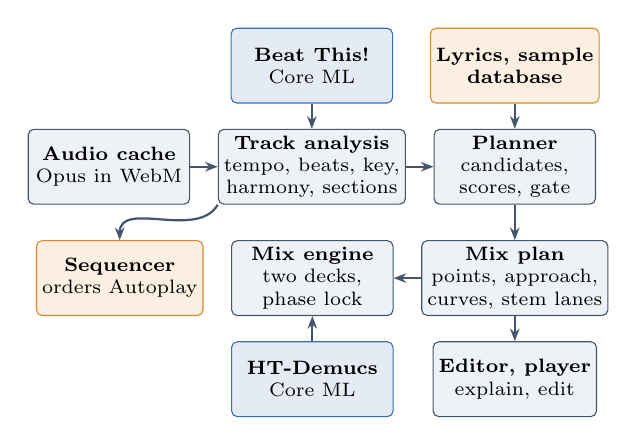
\begin{tikzpicture}[
  font=\scriptsize,
  box/.style={draw=blockline, fill=blockfill, rounded corners=2pt, align=center, minimum width=2.05cm, minimum height=0.95cm, inner sep=2pt},
  model/.style={box, fill=accentA!14, draw=accentA},
  side/.style={box, fill=accentB!14, draw=accentB},
  arr/.style={-{Stealth[length=1.6mm]}, thick, blockline}]
\node[box] (cache) {\textbf{Audio cache}\\Opus in WebM};
\node[box, right=0.35cm of cache] (analysis) {\textbf{Track analysis}\\tempo, beats, key,\\harmony, sections};
\node[model, above=0.32cm of analysis] (beat) {\textbf{Beat This!}\\Core ML};
\node[box, right=0.35cm of analysis] (planner) {\textbf{Planner}\\candidates,\\scores, gate};
\node[side, above=0.32cm of planner] (db) {\textbf{Lyrics, sample}\\\textbf{database}};
\node[box, below=0.45cm of planner] (plan) {\textbf{Mix plan}\\points, approach,\\curves, stem lanes};
\node[box, left=0.35cm of plan] (engine) {\textbf{Mix engine}\\two decks,\\phase lock};
\node[model, below=0.32cm of engine] (stems) {\textbf{HT-Demucs}\\Core ML};
\node[side, left=0.35cm of engine] (seq) {\textbf{Sequencer}\\orders Autoplay};
\node[box, below=0.32cm of plan] (ui) {\textbf{Editor, player}\\explain, edit};
\draw[arr] (cache) -- (analysis);
\draw[arr] (beat) -- (analysis);
\draw[arr] (analysis) -- (planner);
\draw[arr] (db) -- (planner);
\draw[arr] (planner) -- (plan);
\draw[arr] (plan) -- (engine);
\draw[arr] (stems) -- (engine);
\draw[arr] (plan) -- (ui);
\draw[arr] (analysis.south west) to[out=-120,in=90] (seq.north);
\end{tikzpicture}
\caption{Data flow in AutoMix. Blue boxes are neural networks that run through Core ML. Orange
boxes use other information, such as lyrics, a sample database and the queue. Everything runs on
the listener's Mac.}
\label{fig:architecture}
\end{figure}

Fig.~\ref{fig:architecture} shows the parts. When the app caches a song, it analyses the song once
and stores the result on disk under a format version, currently 7. A change to the analysis
therefore invalidates old results. For the playing song and the next one, the planner proposes and
ranks transitions in the background. The player hands the chosen plan to the engine about 30\,s
before its mix point, plus the length of any tempo approach. Planning never delays playback. If no
plan is ready, the next song follows without a gap. The engine writes each cue, start, abandoned
transition and stem decision to a log, \code{mix.log}, so that a developer can explain afterwards
why a transition did not happen. The system is written in Swift and uses only Apple's frameworks.
Accelerate handles signal processing, AVFoundation the audio engine, and Core ML, Apple's on-device
machine-learning framework, the two neural networks.

\begin{table}[t]
\caption{The components of AutoMix}
\label{tab:components}
\centering\footnotesize
\begin{tabular}{@{}>{\raggedright\arraybackslash}p{1.75cm}>{\raggedright\arraybackslash}p{1.75cm}>{\raggedright\arraybackslash}p{4.3cm}@{}}
\toprule
Component & Kind & What it does\\
\midrule
Track analysis & signal processing & finds tempo, beats, bars, key, harmony, tone colour, sections and loudness, once per song\\
Beat model & neural network & corrects beat grids counted at two-thirds or three-halves of the real beat\\
Lyrics and samples & online lookups & line-timed lyrics, and samples documented in MusicBrainz or Genius\\
Planner & search and scoring & proposes up to six transitions for a pair of songs and ranks them\\
Sample gate & logistic model & decides whether a match at another speed is real shared material\\
Tempo limit, ramps & rules from DJ data & keep speed changes between unrelated songs within 20\,\% and two semitones\\
Stem separator & neural network & splits the stretches an overlap covers into vocals, drums, bass and other\\
Mix engine & signal processing & plays two decks in step and applies the plan's curves, approach and stems\\
Sequencer & conditional logit & orders the songs Autoplay adds by how well each mixes out of the last\\
Editor, player & interface & show the plan and its reason, and let the listener change it\\
\bottomrule
\end{tabular}
\end{table}

\subsection{How the parts work together}
Table~\ref{tab:components} lists the components. They act at four moments in a song's life. First,
when the app caches a song, track analysis describes it and the beat model checks its beat grid.
The result is stored, so this happens once. Second, when Autoplay adds songs, the sequencer
re-orders the next five so that each one suits the song before it. Third, as soon as a song becomes
the next one, the planner reads both analyses, any line-timed lyrics and any documented sample link.
It searches for every kind of transition, lets the sample gate reject chance matches at other
speeds, drops Tempo matches beyond the limit, and ranks what remains. In the stem mode, the stem
separator then processes the two stretches the chosen overlap will cover, long before they play.
Fourth, shortly before the mix point, the player hands the plan to the mix engine. The engine moves
the playing song to its new speed and key, starts the next song on the audio clock, keeps the two in
step, applies the volume, equaliser and stem curves, and hands the player over at the midpoint. The
editor and the full-screen player read the same plan the engine performs, so what the listener sees
is what plays.

Fig.~\ref{fig:timeline} follows one approved transition through these steps. MusicBrainz documents
that Kanye West's \emph{Stronger} samples Daft Punk's \emph{Harder, Better, Faster, Stronger}. The
planner therefore searches the two songs at other speeds, finds the sampled passage at 84.2\,\% of
the first song's speed and three semitones lower, and names the plan \q{Known sample, 4 bars}. The
separator processes both sides of the overlap as soon as the plan exists. The engine slows the
first song over 32\,s of its own time, starts \emph{Stronger} in step with it, lets the outgoing
vocals step aside where both songs sing, and swaps the basslines at the midpoint.

\section{Track analysis}\label{sec:analysis}

\subsection{Decoding, loudness and extent}
The app decodes each song to mono at about 12\,kHz, which is enough for rhythm and harmony. It
measures loudness as root-mean-square level in half-second steps. The song's main level is the
median of its middle section. The points where the smoothed level first and last reaches half of
that level mark the end of the intro and the start of the outro. The \emph{energy share} of a time
range is its fraction of the song's total energy. The planner later uses it to price the material
a transition loses or skips.

\subsection{Onsets, tempo and beats}
\emph{Onset strength} measures how sharply new sounds begin. The analysis computes it as spectral
flux, the summed rise in log-compressed magnitude from one spectrum to the next, with a 1024-point
FFT and a hop of 256 samples. It also keeps a separate flux for the band below 200\,Hz. The tempo
comes from the autocorrelation $r$ of the onset envelope over lags from 55 to 210\,BPM. The
analysis scores a candidate lag $\ell$ with
\begin{equation}
s(\ell)=\bigl[r(\ell)+0.7\,r(2\ell)+0.7\,r(4\ell)\bigr]\,
e^{-\frac{1}{2}\left(\log_2(b_\ell/110)/0.9\right)^2},
\end{equation}
where $b_\ell$ is the lag's tempo in BPM. A true beat repeats at the half bar and the bar, so the
terms at two and four beats separate it from a syncopated figure. The log-normal prior prefers
moderate tempi. The tracker then places beats by dynamic programming after Ellis
\cite{ellis2007}. The cumulative score of frame $t$ is its onset strength plus the best earlier
score, less a penalty for departing from the beat period $P$:
\begin{equation}
C(t)=O(t)+\max_{\tau}\Bigl[C(\tau)-100\,\bigl(\ln\tfrac{t-\tau}{P}\bigr)^2\Bigr].
\end{equation}
A least-squares line through the beat times gives the tempo more precisely than any single
interval. The analysis computes a \emph{beat confidence} from the largest normalised
autocorrelation $q$ at the beat, half bar or bar, as $(q-0.3)/0.3$ clipped to the range 0 to 1. It
is low for rubato, ambient and spoken music. Section-aligned blends and matches at another speed
need a confidence of at least 0.5 in both songs, and no plan beat-matches a song below 0.4.

\subsection{Neural beat-error correction}
The built-in tracker has a characteristic failure. It can lock onto a pulse two-thirds or
three-halves as long as the real beat, taking a dotted or triplet figure for the beat. Measured on
the 198 songs of the style groups described in Section~\ref{sec:testing}, this error causes most
of its tempo misses in vocaloid songs. Such a grid puts the beats in the wrong places for any
pairing. AutoMix therefore runs the small checkpoint of Beat This! \cite{beatthis}, which has
2.1\,M parameters and takes about 10\,MB, converted to Core ML. The model reads a log-mel
spectrogram of 22.05\,kHz audio, with 128 mel bands at 50 frames a second, in overlapping 30-second
chunks. It outputs beat and bar-line probabilities. The app computes the spectrogram itself. A
parity test compares the app's beats with those of the original Python model by F-measure, the
harmonic mean of precision and recall when a beat counts as found within 25\,ms of a reference
beat. On 22 November 2026 beats and bar lines both scored 1.000 on six songs, and the model took
3.3 to 4.7\,s per song for songs of 3.5 to 5.3 minutes.

The model's role is deliberately narrow. The analysis re-tracks the onsets at the model's beat
period only when the built-in period is 3/2 or 2/3 of the model's and the two grids agree on fewer
than 80\,\% of beats. It keeps the new grid only if that grid then agrees with the model. The
analysis leaves half- and double-time readings alone, because the planner already compares tempi
across a factor of two and conventions differ by style. Section~\ref{sec:evaluation} shows why. A
larger role for the model produced more accurate grids, but also more fades and changed approved
plans.

\subsection{Bars, key, harmony and sections}
The analysis places bar lines on whichever beat of each four carries the most low-frequency
attack. It finds the key by correlating a chromagram, the pitch-class energy from about C2 to C7,
with the key profiles of Krumhansl and Kessler \cite{krumhansl1982}, and shows it in Camelot notation.
For every beat it stores a 12-dimensional chroma vector for the harmony, and the log energy in
seven bands for the tone colour. The tone-colour bands are an octave wide from 100\,Hz to
3.2\,kHz and standardised per song. It also stores the level of three broad bands. The analysis
finds section boundaries in a bar-by-bar self-similarity matrix scanned with a checkerboard kernel,
which is Foote's novelty measure \cite{foote2000}. It keeps peaks above a threshold that lie at
least four bars apart. Line-timed lyrics show where the singing is when they exist. Otherwise a
mid-band estimate does.

\section{Transition planning}\label{sec:planning}

\subsection{A transition as data}
A transition is a \emph{mix plan}, whose contents Table~\ref{tab:plan} lists. Lanes are
piecewise-linear curves over the overlap's progress $p$, from 0 to 1. The engine turns a volume lane
value $v$ into a gain of $\sin(v\pi/2)$. This equal-power law keeps the combined level steady when
two straight lines cross. An EQ lane value $v$ becomes $-32(1-v)^{1.4}$\,dB, and the filter lane
sweeps a high-pass filter from 30\,Hz to about 5\,kHz.

\begin{table}[t]
\caption{Contents of a mix plan}
\label{tab:plan}
\centering\footnotesize
\begin{tabular}{@{}>{\raggedright\arraybackslash}p{2.3cm}>{\raggedright\arraybackslash}p{5.6cm}@{}}
\toprule
Field & Meaning\\
\midrule
Mix points & the time the playing song starts to leave, and the time the next song enters\\
Length & bars when the beats are matched, seconds when the songs run free\\
Beat periods & the local beat lengths of both songs at the join\\
Approach & the seconds over which the playing song moves to a new speed or key before the overlap\\
Pitch & the semitones the playing song moves\\
Tempo curve & how the shared tempo moves from the playing song's to the next song's across the overlap\\
Lanes on each deck & volume, bass, mids, highs, high-pass filter and echo\\
Stem lanes & the gains of drums, bass, other and vocals on each deck\\
Reason and notes & why the planner chose the plan, shown to the listener\\
\bottomrule
\end{tabular}
\end{table}

\subsection{Candidate families}
For each pair the planner proposes candidates from the families in Table~\ref{tab:families}. It
ranks them by score and keeps up to six, with at most three section-aligned blends and two of each
other kind. It drops near-duplicates, whose mix points lie within 4\,s of each other. A setting
chooses the overlap length, short, medium or long, with targets of 6, 10 and 18\,s. The planner
allows any bar count whose duration lies between 0.45 and 1.8 times the target.

\begin{table}[t]
\caption{Candidate families and their labels}
\label{tab:families}
\centering\footnotesize
\begin{tabular}{@{}>{\raggedright\arraybackslash}p{1.75cm}>{\raggedright\arraybackslash}p{6.15cm}@{}}
\toprule
Label & What it is\\
\midrule
Blend or Mix & an overlap between phrase boundaries with the beats matched; Blend when the equaliser hands the bass over, Mix when the stems do\\
Lyric match & a hand-over on words both songs sing\\
Sound match & a dissolve between passages whose harmony and tone agree\\
Known or Sample match & the next song samples the playing one, possibly at another speed and pitch\\
Tempo match & the harmony agrees only at another speed, in songs the sample gate says share no material\\
Ramp, shown as Blend & songs 12 to 20\,\% apart, eased across before an overlap with the beats matched\\
Fade & a plain fade at the end of the playing song, used as the fallback\\
\bottomrule
\end{tabular}
\end{table}

\subsection{Section-aligned blends}
A blend needs a beat confidence of at least 0.5 in both songs, and tempi within 12\,\% of each other
after allowing for half or double time. The exit lies after a quarter of the playing song, or
later if its intro is long. The entry lies within the first 45\,\% of the next song and at most
100\,s in. Both stretches must consist of regular four-beat bars. For an exit bar, an entry bar and
a length of $L$ bars lasting $s$ seconds against a target of $T$ seconds, the score is
\begin{align}
S={}&1-E^{\text{lost}}_A-1.4E^{\text{skipped}}_B-0.10\left|\log_2\tfrac{s}{T}\right|\nonumber\\
&+0.14\,\beta^{\text{leave}}_A+0.08\,\beta^{\text{start}}_B+0.12\,\beta^{\text{land}}_B+\kappa_A+\kappa_B\nonumber\\
&+0.30(H-0.55)-0.05|k|-0.40\,V\!\left(0.5+0.5\tfrac{s}{T}\right)\nonumber\\
&-0.25\max(0,0.5-H)\tfrac{s}{T}-0.15\min(1,|\lambda_A-\lambda_B|)\nonumber\\
&-1.5\max\!\left(0,|\rho-1|-0.05\right).
\end{align}
Here $E$ are the energy shares of the material lost from the playing song and skipped in the next.
The $\beta$ terms reward leaving on a section boundary and landing the next song's new section as
the old one leaves, which DJs call \q{the classic rule}. The $\kappa$ terms are small beat-clarity
terms. $H$ is the mean harmonic agreement of the overlapping bars after the best pitch shift $k$.
$V$ is the mean product of the two songs' vocal activity, which measures two singers at once. The
$\lambda$ are the levels on either side, and $\rho$ is the ratio of beat periods. The planner takes
a key shift of one or two semitones only when it improves $H$ by more than 0.06 after a penalty of
0.05 a semitone. It then checks the 60 best candidates against the actual beat grids, which must
be steady and clear around both ends. Beat-matching on a mistaken grid sounds worse than not
beat-matching at all.

\subsection{Similarity and samples}
To find passages that sound alike, the planner centres each song's per-beat chroma by removing its
mean, because otherwise songs in related keys look alike everywhere. It resamples the chroma every
0.4\,s. It then compares eight-second windows of the playing song, from a quarter of the way in,
with every alignment in the first two minutes of the next song, and at most 55\,\% of it. The
comparison sums dot products along the diagonals of a matrix. Besides like-for-like matches, the
search tries the next song at other speeds. For each reading of the tempo ratio, counting half and
double time, that lies between 0.62 and 1.6 and more than 12\,\% from 1, it tries several pitch
offsets. These include the offset a record replayed at that speed would have. The planner thus
judges speed and pitch separately, because a producer can slow a sample with or without letting its
pitch fall. A match must stand out from how alike the two songs are in general by at least four
standard deviations.

When no link is documented, a match at another speed must also pass the \emph{sample gate}. The
gate is a logistic model on six standardised measurements $x_i$ of the match. They are the match's
standout within its speed variant, the margin by which one pitch beats the others, and the share of
the playing song that matches somewhere at that speed. The others are the agreement of tone colour,
the distance in semitones from the nearer of the two pitches a sample allows, kept or moved with
the speed, and how close the tempo ratio is to a whole number of semitones. The gate computes
\begin{equation}
z=b+\sum_{i=1}^{6} w_i\,\frac{x_i-\mu_i}{\sigma_i}
\end{equation}
and accepts the match if $z>0.617$. It was trained on 204 positive pairs against 826 negatives,
with folds grouped by song. The positives were sample, interpolation and remix pairs, plus faster
and slower replays of same-speed pairs. The negatives were DJ-adjacent, random and play-history
pairs, also replayed. The strongest cue is the pitch margin, because a real sample matches at one
pitch clearly better than at the others. A link documented in MusicBrainz or Genius names the plan
\q{Known sample} and raises its rank. It does not lower the evidence the planner needs to place the
passage. That was tried, and it invented matches.

\subsection{Tempo matches and ramps}
When the gate rejects a match at another speed, the planner can still offer the move as a \q{Tempo
match}, ranked below what the same tempo offers. Version~2 limits it. The playing song may change
speed by at most 20\,\% and pitch by at most two semitones. The limit came from listening. One plan
took MONTERO to 163\,\% of its speed and up seven semitones to meet Body, which it reached only by
counting Body at double time. The owner heard it and found it unnatural. Planned without the limit
on 22 November, 61 of 91 distinct Tempo matches across the style, common and history pairs moved
tempo by more than 25\,\%, while real DJs stay within 20\,\% in 98.6\,\% of transitions
\cite{kim2020}. Steady songs 12 to 20\,\% apart in tempo
get a \emph{ramp} instead, when no link is documented and nothing lines up at the other tempo. A
ramp is a slow approach to the next song's tempo before a beat-matched overlap near the end.

\subsection{The approach}
Key changes, and the large speed changes of sample matches and Tempo matches, happen on the playing
song before the overlap. They take
\begin{equation}
A=\min\!\left(32,\max\!\left(12,\;8|k|+45|\log_2 r|\right)\right)\ \text{seconds},
\end{equation}
about eight seconds a semitone, where $r$ is the target rate and $k$ the pitch change. The engine
eases the progress $a$ through the approach, from 0 to 1, with $e(a)=6a^5-15a^4+10a^3$, a curve with
no audible start or stop. It applies the eased value geometrically to the rate, as $r^{e}$, and
linearly to the pitch, as $k\,e$. A ramp moves more slowly still, over $220\,g$ seconds for a tempo
gap $g$, between 16 and 45\,s. Fig.~\ref{fig:timeline} shows the approach and overlap of an approved
plan. Within a blend with the beats matched, the two tempi differ by at most 12\,\%. In overlaps
of 12\,s or more, they glide together across the middle 70\,\% of the overlap. Shorter overlaps
hold the old tempo, and the new song eases to its own tempo afterwards.

\begin{figure}[t]
\centering
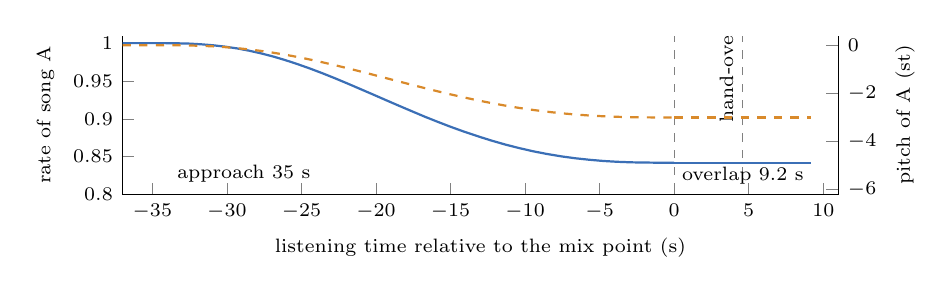
\begin{tikzpicture}
\begin{axis}[
  width=0.88\columnwidth, height=3.6cm,
  xmin=-37, xmax=11, ymin=0.80, ymax=1.01,
  xlabel={listening time relative to the mix point (s)}, ylabel={rate of song A},
  ylabel style={font=\scriptsize}, xlabel style={font=\scriptsize},
  tick label style={font=\scriptsize},
  axis y line*=left, axis x line*=bottom,
  every axis plot/.append style={thick}]
\addplot[accentA] coordinates {(-37,1) (-34.95,1.0000) (-34.15,1.0000) (-33.35,0.9998) (-32.55,0.9994) (-31.75,0.9985) (-30.94,0.9972) (-30.14,0.9954) (-29.34,0.9931) (-28.53,0.9901) (-27.72,0.9865) (-26.91,0.9824) (-26.09,0.9776) (-25.27,0.9723) (-24.45,0.9666) (-23.62,0.9604) (-22.78,0.9538) (-21.94,0.9469) (-21.09,0.9397) (-20.23,0.9324) (-19.37,0.9250) (-18.50,0.9176) (-17.63,0.9103) (-16.75,0.9030) (-15.86,0.8960) (-14.96,0.8892) (-14.06,0.8828) (-13.15,0.8768) (-12.23,0.8711) (-11.31,0.8659) (-10.39,0.8613) (-9.46,0.8571) (-8.52,0.8535) (-7.58,0.8504) (-6.64,0.8479) (-5.69,0.8459) (-4.75,0.8443) (-3.80,0.8432) (-2.85,0.8425) (-1.90,0.8422) (-0.95,0.8420) (0.00,0.8420)};
\addplot[accentA] coordinates {(0,0.842) (9.2,0.842)};
\draw[dashed, gray] (axis cs:0,0.826) -- (axis cs:0,1.01);
\draw[dashed, gray] (axis cs:4.6,0.826) -- (axis cs:4.6,1.01);
\node[font=\scriptsize, anchor=south west] at (axis cs:-34,0.803) {approach 35 s};
\node[font=\scriptsize, anchor=south] at (axis cs:4.6,0.801) {overlap 9.2 s};
\node[font=\scriptsize, anchor=south, rotate=90] at (axis cs:4.6,0.958) {hand-over};
\end{axis}
\begin{axis}[
  width=0.88\columnwidth, height=3.6cm,
  xmin=-37, xmax=11, ymin=-6.2, ymax=0.4,
  axis y line*=right, axis x line=none, ylabel={pitch of A (st)},
  ylabel style={font=\scriptsize}, tick label style={font=\scriptsize},
  every axis plot/.append style={thick}]
\addplot[accentB, dashed] coordinates {(-37,0) (-34.95,-0.000) (-34.15,-0.000) (-33.35,-0.003) (-32.55,-0.011) (-31.75,-0.026) (-30.94,-0.048) (-30.14,-0.080) (-29.34,-0.122) (-28.53,-0.174) (-27.72,-0.237) (-26.91,-0.311) (-26.09,-0.395) (-25.27,-0.489) (-24.45,-0.593) (-23.62,-0.706) (-22.78,-0.826) (-21.94,-0.952) (-21.09,-1.084) (-20.23,-1.221) (-19.37,-1.360) (-18.50,-1.500) (-17.63,-1.640) (-16.75,-1.779) (-15.86,-1.916) (-14.96,-2.048) (-14.06,-2.174) (-13.15,-2.294) (-12.23,-2.407) (-11.31,-2.511) (-10.39,-2.605) (-9.46,-2.689) (-8.52,-2.763) (-7.58,-2.826) (-6.64,-2.878) (-5.69,-2.920) (-4.75,-2.952) (-3.80,-2.974) (-2.85,-2.989) (-1.90,-2.997) (-0.95,-3.000) (0.00,-3.000)};
\addplot[accentB, dashed] coordinates {(0,-3) (9.2,-3)};
\end{axis}
\end{tikzpicture}\\[2pt]
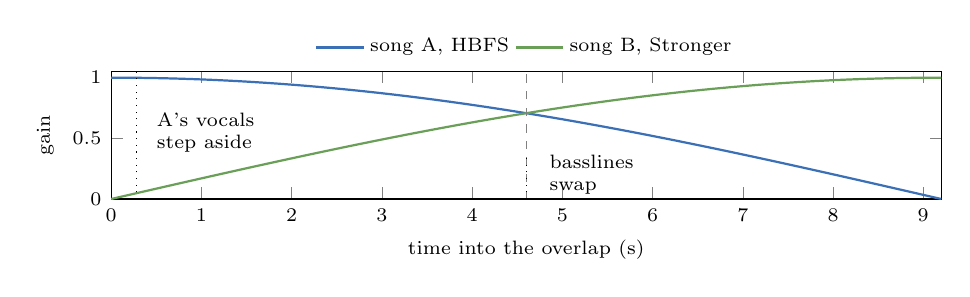
\begin{tikzpicture}
\begin{axis}[
  width=\columnwidth, height=3.2cm,
  xmin=0, xmax=9.2, ymin=0, ymax=1.05,
  xlabel={time into the overlap (s)}, ylabel={gain},
  ylabel style={font=\scriptsize}, xlabel style={font=\scriptsize},
  tick label style={font=\scriptsize},
  legend style={font=\scriptsize, at={(0.5,1.03)}, anchor=south, legend columns=2, draw=none},
  every axis plot/.append style={thick}]
\addplot[accentA, domain=0:9.2, samples=60] {sin(deg((1 - x/9.2)*pi/2))};
\addplot[accentC, domain=0:9.2, samples=60] {sin(deg((x/9.2)*pi/2))};
\legend{{song A, HBFS},{song B, Stronger}}
\draw[dashed, gray] (axis cs:4.6,0) -- (axis cs:4.6,1.05);
\draw[dotted, black] (axis cs:4.6,0) -- (axis cs:4.6,0.35) node[font=\scriptsize, anchor=west, align=left] at (axis cs:4.75,0.2) {basslines\\swap};
\draw[dotted, black] (axis cs:0.28,0) -- (axis cs:0.28,1.05);
\node[font=\scriptsize, anchor=west, align=left] at (axis cs:0.4,0.55) {A's vocals\\step aside};
\end{axis}
\end{tikzpicture}
\caption{The approved plan from \emph{Harder, Better, Faster, Stronger} by Daft Punk into
\emph{Stronger} by Kanye West, which samples it. The app labels it \q{Known sample, 4 bars}. In the top
panel, the playing song moves to 84.2\,\% of its speed, shown solid, and three semitones down, shown
dashed. The move takes 32\,s of the song's own time, about 35\,s of listening because the song
slows, and the song holds both through the overlap. The bottom panel shows the equal-power volume
curves over the 9.2\,s overlap. With stems on, the outgoing vocals stepped aside 3\,\% into the overlap, and the
basslines swap at the midpoint, where the player hands over to the next song.}
\label{fig:timeline}
\end{figure}

\subsection{Stem lanes}
In the stem mode, the planner gives stem lanes to plans of at least two bars with the beats
matched, following Mosaikbox \cite{mosaikbox}. The basslines swap at the middle of the overlap, so
two never play at once. In blends of different songs, the new drums rise over the second quarter
while the old ones fall to 0.4 and then 0.1. If both songs sing at once, the outgoing vocals step
aside, and the engine decides the exact moment at playback on the separated vocals, as
Section~\ref{sec:engine} describes. A lyric match keeps both vocals, because the shared words are
the reason for the match.

\section{Playback engine}\label{sec:engine}

\subsection{Decks and scheduling}
The engine has two decks that feed one mixer, followed by a master equaliser and limiter. Each deck
decodes Opus audio from WebM files and passes it through Apple's time-pitch unit, which sets a rate
from 0.5 to 2 and the pitch independently. A four-band equaliser and a delay for echo follow. The
approach follows the playing deck's position, so the listener can pause and seek during it safely.
The engine cues and buffers the incoming deck beforehand. It starts the deck at an exact host time,
the remaining time to the mix point less the output latency and the time-stretcher's latency.

\subsection{Phase lock}
A phase lock absorbs small timing errors at the start and tempo drift. After 3\,\% of the overlap,
the engine compares how many beats each deck has travelled since its mix point,
$e=\Delta b_B-\Delta b_A$. If $|e|$ is under 0.45 beats, the engine updates a smoothed error and
adjusts the incoming deck's rate:
\begin{equation}
d\leftarrow d+0.08(e-d),\qquad
r_B\leftarrow r_B\,\bigl(1+\operatorname{clip}(-0.6\,d,\pm0.025)\bigr).
\end{equation}

\subsection{Hand-over and settling}
At the midpoint of the overlap the player switches to the incoming song. Its title, position and
controls take over, and the player tells listening services that it is playing. When the overlap
ends, a song left at another speed or pitch eases back to its own along the curve $3a^2-2a^3$ over
$\max(8,\,150|r-1|,\,6|k|)$ seconds, at most 24. If the next song is not ready at the mix point, the
engine waits. More than 1.5\,s past the mix point, it abandons the transition and the songs follow
without a gap. A song loaded before the listener switched AutoMix on cannot change speed, so its
planned move falls back to a cross-fade of the same length. Since version~2, a seek after the
engine has cued a transition hands the transition to the engine again. Before, the transition was
lost and the next song followed after a gap.

\subsection{Stems at playback}
The Core ML conversion of HT-Demucs \cite{htdemucs} contains only the network. The app performs
what demucs 4.0.1 does around it, which is reflect padding, a normalised 4096-point STFT with a hop
of 1024 and a periodic Hann window, its inverse, and 7.8\,s segments cross-faded with triangular
weights. Half precision converts but gives wrong stems, so the model runs in single precision. The
app separates only the two stretches an overlap covers, as soon as the planner decides the
transition, and caches the result. On the test Mac the model loaded in 1.3\,s, and a 7.8\,s segment
took 0.68\,s, the first run included. The app still loads the model and separates one silent segment
at launch, so that a slow first run never falls on a transition. Each deck plays
\begin{equation}
y(t)=x(t)-\sum_{s}\bigl(1-g_s(p)\bigr)\,\hat{x}_s(t),
\end{equation}
removing $1-g_s$ of each separated stem $\hat{x}_s$ from what it reads. The stems line up with
playback to the sample. Opus decoding runs 3.5\,ms ahead of playback's packet times, and the app
corrects that offset.

Three timing rules came from a listening test in which vocals bled through. First, decks read about
three seconds ahead of what is heard, and stems change only what a deck reads after they are set.
Stems that arrive late therefore start from the deck's read position and fade in over a beat.
Second, a side whose stems were not in place when the overlap began swaps its bass on the equaliser
instead, because a stem plan switches the equaliser's bass swap off. Third, the engine decides the
vocal hand-over on the separated vocal stems. Where both songs sing at once for more than a second,
the outgoing vocals fade over half a beat on the last beat before the incoming vocals start. The
engine takes vocal segments from the vocal stem by Mosaikbox's rule. Silences of at least 1\,s
below $-40$\,dBFS split the stem, and the engine keeps parts of at least 0.4\,s.

\section{Ordering the queue}\label{sec:sequencer}

Autoplay is YouTube Music's continuation of the queue with recommended songs. When it adds songs,
AutoMix fetches and analyses the next five ahead and re-orders them so that each one mixes well out
of the song before it. That song is one the listener chose with Play Next when one is waiting.
AutoMix never moves songs queued by hand, albums or playlists, and it leaves the next song alone once
its transition is near. The fit of a candidate is the logistic function of a sum of learned
log-odds weights over features of the pair, which Table~\ref{tab:sequencer} lists. The sequencer
subtracts 0.03 for each place the candidate stands behind the first candidate in Autoplay's own
order. It places the best fit next and continues the chain from it. The weights come from a
conditional logit model. In it, each of 501 next songs in 28 DJ-made sequences competed against
four others from the same sequence. The sequences are 12 Spotify \q{Mixed By} playlists and 16
discs or parts of 6 DJ-mixed albums, the ones with enough songs the app could analyse.

\begin{table}[t]
\caption{Learned sequencer weights in log-odds}
\label{tab:sequencer}
\centering\footnotesize
\begin{tabular}{@{}lr@{\hspace{1.2em}}lr@{}}
\toprule
Feature & Weight & Feature & Weight\\
\midrule
tempo gap per 12\,\% & $-0.632$ & compatible key & $0.162$\\
gap beyond 12\,\% & $-0.150$ & diagonal key step & $-0.111$\\
free tempo & $-0.985$ & 1-semitone shift & $0.107$\\
half or double time & $0.301$ & 2-semitone shift & $-0.253$\\
same artist & $0.214$ & key clash & $0.063$\\
loudness per 6\,dB & $-0.177$ & key unknown & $0.032$\\
\bottomrule
\end{tabular}
\end{table}

\section{Interface and explanation}\label{sec:interface}

\begin{figure}[t]
\centering
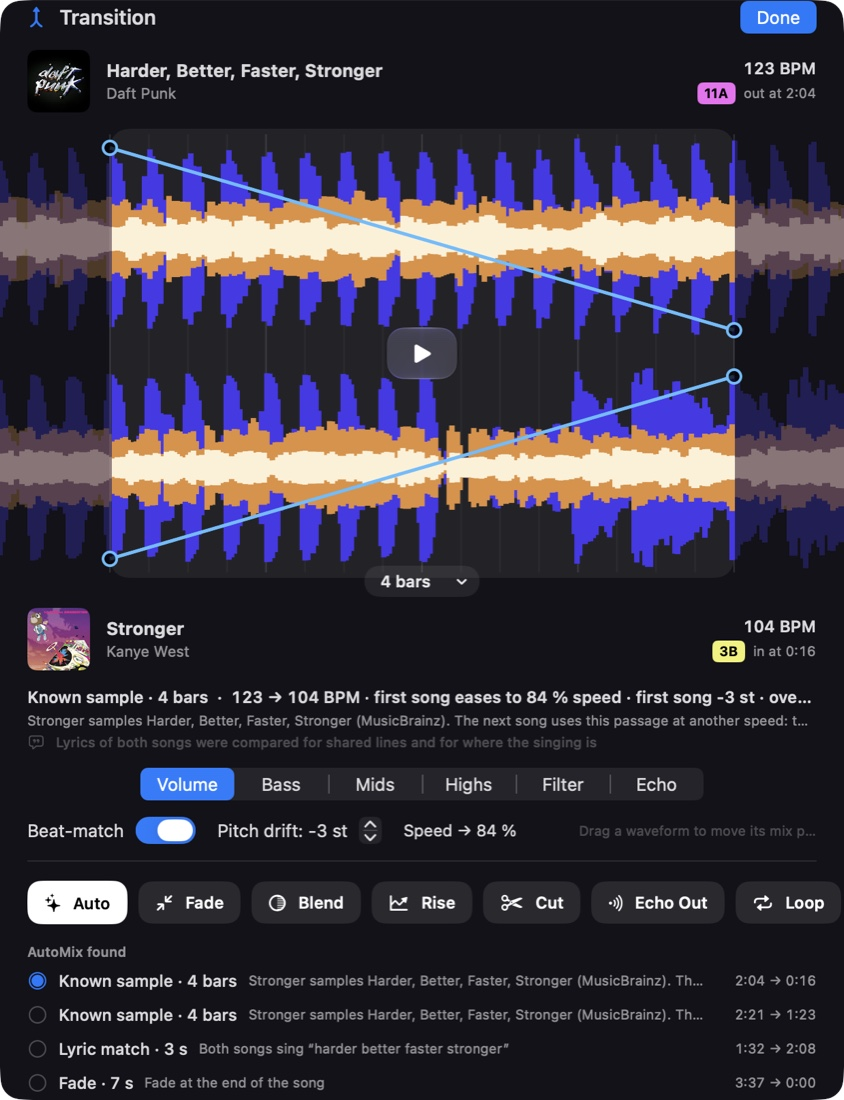
\includegraphics[width=0.84\columnwidth]{figures/mix-editor.jpg}
\caption{The transition editor for the plan of Fig.~\ref{fig:timeline}. It shows both songs'
waveforms in three bands with the volume curves, their tempo and Camelot key, the plan's
description, the lane selector, the presets, and AutoMix's other proposals, which include a lyric
match on a line both songs sing. The screenshot is of the running application.}
\label{fig:editor}
\end{figure}

Every plan carries a label and a sentence saying why the planner chose it. The transition editor
in Fig.~\ref{fig:editor} shows both songs' waveforms aligned at the mix point. The listener can
drag a waveform to move its mix point, edit any lane's curve, apply a preset or pick another
proposal. The presets are Fade, Blend, Rise, Cut, Echo Out and Loop. Trying a proposal or preset
affects only the current play of the pair, and the app saves hand edits per pair of songs. In the
full-screen player of Fig.~\ref{fig:player}, the next song's cover slides in beside the playing one
when a transition begins, and the background blends the colours of both covers. At the hand-over
the old cover slides away and the new one moves to the centre. The playback controls stay in place
throughout.

\begin{figure}[t]
\centering
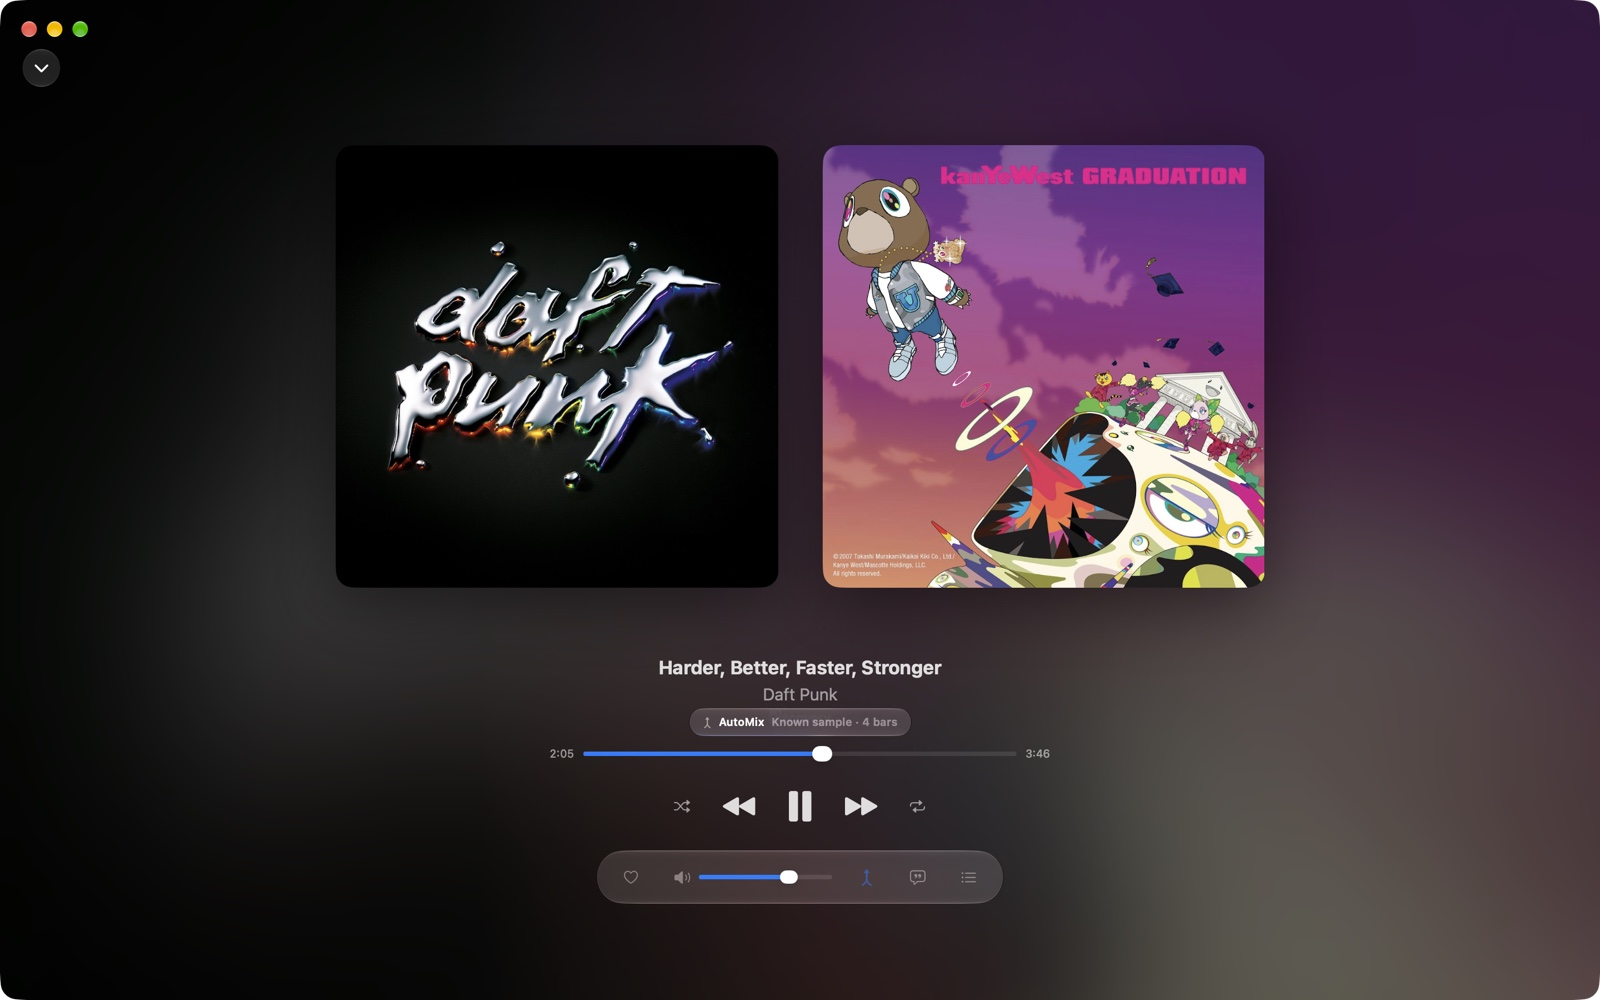
\includegraphics[width=\columnwidth]{figures/player-transition.jpg}
\caption{The full-screen player during the first half of the transition of
Fig.~\ref{fig:timeline}. The screenshot is of the running application.}
\label{fig:player}
\end{figure}

\section{Testing method}\label{sec:testing}

People judge transitions by ear, but no one can listen to every pair after every change. The
project therefore tests the system at several levels, which Table~\ref{tab:tests} summarises. The
central safeguard is a set of \emph{approved reference pairs}, transitions the owner approved by
ear. Their plans, as the audit writes them out, must stay byte-identical after any change that is
not meant to alter them. The pairs include \emph{P.Y.T.} into \emph{Good Life}, which samples it at
two-thirds speed but higher in pitch.

\emph{Parity tests} check the converted models against the originals. They compare the beat model's
beats and bar lines with the Python implementation, and the separated stems with HT-Demucs in
PyTorch. They score the stems by signal-to-distortion ratio, or SDR, with a pass mark of 40\,dB.

\emph{Audits} plan hundreds of pairs from cached analyses with a fixed random seed, so that runs
before and after a change plan the same pairs. They cover 200 pairs drawn within and across seven
style groups of 198 songs in all, which are electronic, hip-hop, J-pop, pop, rock, vocaloid and
other. They also cover 37 well-known sample pairs and blends, the approved pairs, and pairs from the
owner's listening history. The audits report how often plans beat-match or fade, how far they
stretch, where they enter and leave, and whether the two songs' kick drums actually line up through
the plan. The kick check uses each song's own low-band onsets below 150\,Hz rather than the beat
grids the plan was built from, so it can catch a grid that sits on the snare. The planner never
sees the style labels.

\emph{Behavioural suites} drive the real player. They run offline feature checks, six of them on
stem timing. They check the order of Play Next, radio and Autoplay songs, and mixing into a video's
audio release. The suites render real transitions through the engine, muted, and check the log
lines. One check confirms that stems separated ahead are ready as soon as the engine cues the
transition, and another that late stems fall back to the equaliser. A window test plays a transition
in the real full-screen player and records the states of the covers.

\begin{table}[t]
\caption{Checks run on the version described, on 22 November 2026}
\label{tab:tests}
\centering\footnotesize
\begin{tabular}{@{}>{\raggedright\arraybackslash}p{3.1cm}>{\raggedright\arraybackslash}p{4.8cm}@{}}
\toprule
Check & Result\\
\midrule
10 approved pairs & byte-identical to the previous run, with and without stems\\
Feature checks & 47 of 47 pass, 6 of them on stem timing\\
Play Next and mixing & 17 pass; 3 fail on an outdated label\\
Video audio release & 5 pass; 1 fails on the same label\\
Radio and queue order, live & 14 of 14 pass\\
Beat model parity with Python & beat and bar F 1.000 on 6 songs\\
Stem parity with PyTorch & worst stem 112.0\,dB SDR, pass mark 40\,dB\\
Stems separated ahead & ready 0.0\,s after cueing, before the overlap\\
Stems late & EQ bass swap, then stems after 3.9\,s, faded in from the read position\\
Transition view & both covers, then the hand-over, in a real transition\\
Page buttons over the player & hidden while it is open, back when it closes\\
\bottomrule
\end{tabular}
\end{table}

The four failing checks in Table~\ref{tab:tests} expect the label \q{Sample match} where the planner
now says \q{Known sample}, because it finds a database link. The checks predate this version, and
the plans themselves are the approved ones.

\section{Evaluation}\label{sec:evaluation}

All results in this section are measurements. None of them replaces listening, and no formal
listening study has been run, as Section~\ref{sec:limits} discusses.

\subsection{Beat model}
Fig.~\ref{fig:beat} compares three roles for the beat model. For each role, the current build
analysed the 198 songs of the style groups from scratch on 22 November 2026 and then planned the
same pairs. Accuracy is measured against reference labels made by the large Beat This! model, which
are a development reference rather than ground truth. Without the model, the built-in tracker
scores a beat F-measure of 0.796 and a downbeat F-measure of 0.431. Replacing its grid with the
model's raises these to 0.953 and 0.899. It also changes 9 of the 10 approved plans and raises the
share of fades from 26 to 37\,\% among the style pairs and from 19 to 27\,\% among 242 pairs
from the owner's listening history. The planner was tuned on the built-in grids, whose bars always
come in fours, so more accurate grids alone did not produce better mixes. The shipped role
corrects only 2:3 pulse errors. It gives 0.814 overall, raises vocaloid songs from 0.668 to 0.724
and their correct tempi from 46 to 56\,\%, and leaves the approved plans byte-identical. A fourth
role measured on 21 November, which also corrected the tempo octave and the bar phase, is no longer
in the code, so it is not reported here.

\begin{figure}[t]
\centering
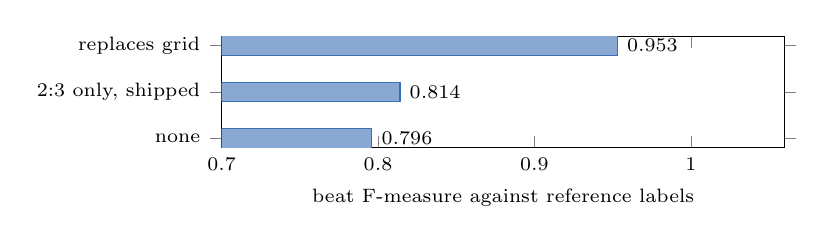
\begin{tikzpicture}
\begin{axis}[
  xbar, width=0.72\columnwidth, height=3.0cm,
  xmin=0.7, xmax=1.06, bar width=7pt, xtick={0.7,0.8,0.9,1.0},
  symbolic y coords={none,{2:3 only, shipped},{replaces grid}},
  ytick=data, y tick label style={font=\scriptsize},
  xlabel={beat F-measure against reference labels}, xlabel style={font=\scriptsize},
  tick label style={font=\scriptsize},
  nodes near coords, nodes near coords style={font=\scriptsize},
  every node near coord/.append style={/pgf/number format/fixed,/pgf/number format/precision=3}]
\addplot[fill=accentA!60, draw=accentA] coordinates {(0.796,none) (0.814,{2:3 only, shipped}) (0.953,{replaces grid})};
\end{axis}
\end{tikzpicture}
\caption{Beat accuracy for each role of the beat model on the 198 style-group songs, against
labels made by the large Beat This! model, measured on 22 November 2026. The most accurate role gave
more fades and changed 9 of the 10 approved plans, so it was not shipped.}
\label{fig:beat}
\end{figure}

\subsection{Sample gate}
The current build computed the gate's measurements again for 1,040 pairs that have a match at
another speed, 204 of them real shared material. Held out by song over repeated folds, a gate
trained in the shipped way separates the two with an area under the ROC curve of 0.713, with a
standard deviation of 0.009. A model on the previous rule's single measure, how far the match
stands out, scores 0.644. The previous rule itself, a match standing 4.5 standard deviations
above the same-speed alignments, caught 89\,\% of real matches but fired on 69\,\% of unrelated
pairs. At its threshold, the shipped gate passes 7.2\,\% of the unrelated pairs and 42.6\,\% of the
real matches. The threshold treats a missed sample as the lesser error, because a missed sample
falls back to a blend, while a false one brings a large speed change between unrelated songs.
Among the 200 style pairs, unconfirmed \q{Sample match} plans fell from 33\,\% under the
previous rule to 6\,\%, and among the 242 history pairs from 24 to 5\,\%.

\subsection{Limit on Tempo matches}
Fig.~\ref{fig:types} shows the plans chosen for the 200 style pairs without and with the limit of
20\,\% and two semitones. Both runs used the same analyses, made from scratch by the current build
on 22 November 2026. Tempo matches fell from 49 to 10, and none of them
now moves tempo by more than 20\,\%. Sound matches rose from 14 to 27 and fades from 29 to 53. Plans
that stretch either song by more than 20\,\% fell from 47 to 10. The remaining ten are seven sample
matches and three ramps. A ramp's gap of up to 20\,\% is measured against the playing song's tempo,
so a ramp can speed that song up by as much as 25\,\%. Beat-synchronised plans fell from 162 to 125.
Of the 37 well-known sample pairs and blends, only two plans changed, both of them Tempo matches.
One became a fade and the other a blend. Among the 242 history pairs, Tempo matches fell from 41
to 8 and fades rose from 23 to 45. The approved pairs were unchanged, and MONTERO into Body became
a seven-second fade. The owner listened to it again on 22 November and judged that it now sounds
good.

\begin{figure}[t]
\centering
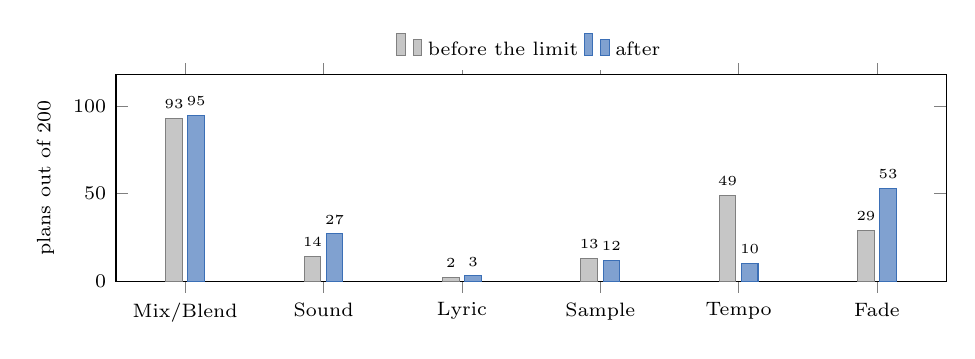
\begin{tikzpicture}
\begin{axis}[
  ybar, width=\columnwidth, height=4.2cm, bar width=6pt,
  ymin=0, ymax=118,
  symbolic x coords={Mix/Blend,Sound,Lyric,Sample,Tempo,Fade},
  xtick=data, x tick label style={font=\scriptsize},
  ylabel={plans out of 200}, ylabel style={font=\scriptsize},
  tick label style={font=\scriptsize},
  nodes near coords, nodes near coords style={font=\tiny},
  legend style={font=\scriptsize, at={(0.5,1.02)}, anchor=south, legend columns=2, draw=none},
  enlarge x limits=0.1]
\addplot[fill=gray!45, draw=gray] coordinates {(Mix/Blend,93) (Sound,14) (Lyric,2) (Sample,13) (Tempo,49) (Fade,29)};
\addplot[fill=accentA!65, draw=accentA] coordinates {(Mix/Blend,95) (Sound,27) (Lyric,3) (Sample,12) (Tempo,10) (Fade,53)};
\legend{before the limit, after}
\end{axis}
\end{tikzpicture}
\caption{Plan types for 200 style-group pairs before and after limiting Tempo matches to 20\,\%
speed and two semitones, with the same analyses and pairs. Mix and Blend include ramps.}
\label{fig:types}
\end{figure}

\subsection{Stems}
Fig.~\ref{fig:sdr} shows the parity of the Core ML separator with PyTorch on one 7.8\,s segment.
Every stem is far above the 40\,dB pass mark. Separating a 20\,s stretch of audio at 48\,kHz took
2.8\,s, and the app starts as soon as the planner decides a transition, long before the overlap.
Without lyrics, the planner's own estimate of where the singing is was wrong on 44\,\% of bars
against the separated vocals of 88 songs, with a pooled area under the ROC curve of 0.642. The vocal
hand-over therefore waits for the stems. A check on the six songs of the three approved sample pairs
measured how deep the separation goes, by separating the processed audio again. One pass left the
vocals 44 to 57\,dB below their original level, and a second subtraction pass gained 0 to 7\,dB, so
the app does not make one.

\begin{figure}[t]
\centering
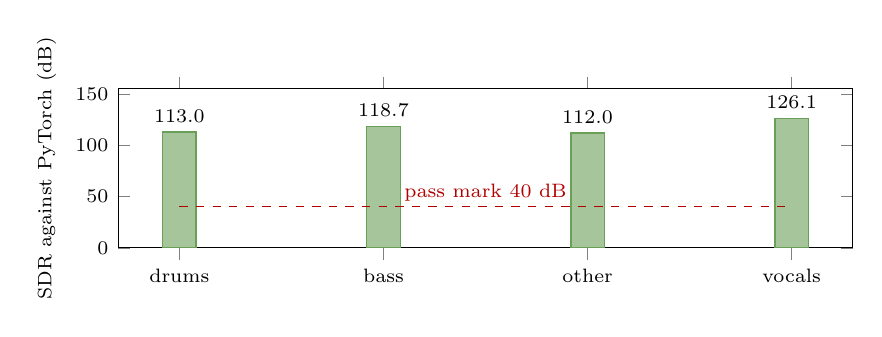
\begin{tikzpicture}
\begin{axis}[
  ybar, width=0.9\columnwidth, height=3.6cm, bar width=12pt,
  ymin=0, ymax=155,
  symbolic x coords={drums,bass,other,vocals},
  xtick=data, tick label style={font=\scriptsize},
  ylabel={SDR against PyTorch (dB)}, ylabel style={font=\scriptsize},
  nodes near coords, nodes near coords style={font=\scriptsize},
  every node near coord/.append style={/pgf/number format/fixed,/pgf/number format/fixed zerofill,/pgf/number format/precision=1}]
\addplot[fill=accentC!60, draw=accentC] coordinates {(drums,113.0) (bass,118.7) (other,112.0) (vocals,126.1)};
\draw[dashed, red!70!black] (axis cs:drums,40) -- (axis cs:vocals,40);
\node[font=\scriptsize, text=red!70!black, anchor=south, fill=white, inner sep=1pt] at (rel axis cs:0.5,0.27) {pass mark 40 dB};
\end{axis}
\end{tikzpicture}
\caption{Agreement of the app's Core ML stem separation with HT-Demucs in PyTorch, per stem, as
signal-to-distortion ratio on one 7.8\,s segment on 22 November 2026.}
\label{fig:sdr}
\end{figure}

\subsection{Queue ordering}
On sequences held out from training, the DJ's actual next song ranked first among five in
29.9\,\% of cases with the learned weights. The hand-set weights they replaced, 0.5 for tempo, 0.3
for key and 0.2 for artist, scored 27.8\,\%, and chance is 20\,\%. Mean reciprocal rank rose by
0.020, but its 95\,\% bootstrap interval, from $-0.002$ to 0.040, includes zero. On 28 sequences
and 501 transitions the gain is therefore not yet clear. Retraining on the current analyses moves
no weight by more than 0.03, and the weights still suggest that DJs weigh tempo most and key far
less than the hand-set weights assumed.

\section{Limitations and future work}\label{sec:limits}

\subsection{Limitations of AutoMix}
The most important limitation is that no formal listening study has been run. The ten approved
pairs encode one listener's judgement, and every other result in Section~\ref{sec:evaluation}
measures plans rather than how they sound. The audits' kick check is only a rough guide, because it
flags 3 of the 9 approved plans it can check.

Beat and bar analysis remains the weakest link. Without the beat model, the built-in tracker finds
the right tempo in 46\,\% of the vocaloid songs, and in 56\,\% with it. Bar lines are worse than
beats in every style group, with a downbeat F-measure of 0.439 overall. The planner was tuned on the
built-in grids, whose bars always come in fours, so a more accurate grid did not help. Replacing the
grid with the model's raised the downbeat F-measure to 0.899, but it changed 9 of the 10 approved
plans and raised fades among the style pairs from 26 to 37\,\%. All of these accuracy figures rest
on labels made by a larger model, not on labels checked by ear.

The planner places singing from line-timed lyrics, and without them from the share of each bar's
energy in the middle band. Measured against the separated vocals of 88 songs, that estimate is wrong
on 44\,\% of bars. The blend score's penalty for clashing vocals uses it, so the planner can still
rank a blend as if two singers clashed when they do not, or the reverse. The stems correct the
vocal hand-over at playback, but not the choice of plan.

The sample gate catches about 43\,\% of real matches at another speed and passes about 7\,\% of
unrelated pairs, so it misses more samples than it finds. Its 204 positive pairs come mostly from
hip-hop and electronic music. Documented links depend on what MusicBrainz and Genius record.

The key is one estimate per song, from profiles built on listeners' judgements of Western tonal
music \cite{krumhansl1982}. A song that changes key, or whose scale the profiles do not describe,
can be given the wrong key, and the planner has no separate key for the intro or the outro.

The limit on Tempo matches trades large speed changes for fades, and no listener has yet judged
the remaining Tempo matches or the ramps. The engine changes speed and pitch with Apple's
time-pitch unit, whose sound at large changes the project has not measured.

Stem separation runs only around transitions and needs a model of about 200\,MB. Its parity
tests compare the app with PyTorch rather than with true stems, so they show that the conversion is
faithful, not how clean the stems are. Separating the processed audio again still finds vocal
energy 44 to 57\,dB below the original vocals. HT-Demucs cannot remove vocals that it has itself put in the \q{other} stem.

The learned queue order puts the DJ's choice first slightly more often than the hand-set weights,
but the 95\,\% interval of the gain includes zero. Finally, a transition needs both songs'
analyses, so when the next song has not been fetched and analysed in time, the songs follow without
a gap.

\subsection{Limitations of research on automatic DJ mixing}
The field has no agreed objective measure of transition quality. The authors of Mosaikbox point to
\q{the subjective nature of mixes} and to the lack of ground-truth corpora for the similarity of
songs, and they evaluate with a listening experiment \cite{mosaikbox}. Without a shared benchmark,
published systems cannot be compared directly, and this report cannot compare AutoMix with them.

Listening studies in the field are small and narrow. Mosaikbox's study had 30 participants, mainly
academics aged 23 to 30, of whom 8 had DJ experience. All of its songs were drum and bass, chosen
because most participants knew the genre \cite{mosaikbox}. The fully automatic system of Vande Veire
and De Bie also works on drum and bass \cite{vandeveire2018}. Such results may not carry over to
pop, hip-hop or J-pop, where vocals dominate.

What is known about real DJ practice comes mostly from electronic dance music. The 1,557 mixes that
Kim \emph{et al.}\ analysed are mostly house and trance, and their alignment method did not work
well for some genres such as techno \cite{kim2020}. AutoMix's 20\,\% limit on tempo changes rests on
those statistics, and whether listeners of other styles accept the same changes is unknown.

Copyright limits the data. Kim \emph{et al.}\ used mix metadata that 1001Tracklists provided with
permission, and they ask researchers who want it to contact 1001Tracklists \cite{kim2020}. The
audio of commercial songs cannot be shared at all. The authors of Mosaikbox count it an advantage
that their rule-based design needs no training on copyrighted music \cite{mosaikbox}. Learned parts
therefore train on small private sets, as AutoMix's sample gate and sequencer do.

The commercial services that mix songs automatically publish neither their methods nor any
evaluation \cite{spotifymix,applemix}, so research systems cannot be measured against them.

\subsection{Future work}
The next step is a listening study that rates transitions with and without each component, like
that of Mosaikbox but across styles. Beats and bar lines need labels checked by ear. Adapting the
planner to grids whose bars vary would let the beat model take a larger role. Further work includes
measuring singing on the stems during analysis, local keys at the intro and outro, drum-pattern
similarity for the drum rule, a stronger vocal model, and a larger and more varied set of DJ
sequences for the queue order.

\section{Conclusion}

AutoMix plans, explains and performs DJ-style transitions entirely on a personal computer. Classic
signal processing does most of the work. Neural networks have two narrow roles. One corrects a
single class of beat error, because larger roles for the beat model gave more accurate grids but
more fades. The other separates stems for a few seconds around each transition, following rules
that a listening study found to help \cite{mosaikbox}. Learned models replaced hand-set rules where
reference data existed, and the limit on speed changes follows what real DJs do. A small set of
approved transitions, parity tests against the original models, and audits over hundreds of pairs
made every change measurable, while listening remains the final judge.

\section*{Acknowledgment}
The project's owner directed this work, set its requirements and judged the transitions by ear.
The client follows the design of the open-source Android app Metrolist \cite{metrolist}. The beat
model \cite{beatthis} and the stem model \cite{htdemucs} are released under the MIT licence.

\begin{thebibliography}{99}

\bibitem{spotifymix}
Spotify, \q{Mix your favorite playlists seamlessly by adding your own transitions,} Spotify
Newsroom, Aug.\ 19, 2025. Accessed: Nov.\ 22, 2026. [Online]. Available:
\url{https://newsroom.spotify.com/2025-08-19/mix-your-favorite-playlists-seamlessly-by-adding-your-own-transitions/}

\bibitem{applemix}
Apple, \q{Apple services deliver powerful features and intelligent updates to users this fall,}
Apple Newsroom, Jun.\ 2025. Accessed: Nov.\ 22, 2026. [Online]. Available:
\url{https://www.apple.com/my/newsroom/2025/06/apple-services-deliver-powerful-features-and-intelligent-updates-to-users-this-fall}

\bibitem{metrolist}
Metrolist Group, \q{Metrolist,} GitHub repository. Accessed: Nov.\ 22, 2026. [Online]. Available:
\url{https://github.com/MetrolistGroup/Metrolist}

\bibitem{kim2020}
T.~Kim, M.~Choi, E.~Sacks, Y.-H.~Yang, and J.~Nam, \q{A computational analysis of real-world DJ
mixes using mix-to-track subsequence alignment,} in \emph{Proc.\ 21st Int.\ Soc.\ Music Inf.\
Retrieval Conf.\ (ISMIR)}, 2020, pp.~764--770, doi: 10.5281/zenodo.4245544.

\bibitem{vandeveire2018}
L.~Vande~Veire and T.~De~Bie, \q{From raw audio to a seamless mix: Creating an automated DJ system
for Drum and Bass,} \emph{EURASIP J.\ Audio, Speech, Music Process.}, vol.~2018, no.~1,
Art.~no.~13, Sep.\ 2018, doi: 10.1186/s13636-018-0134-8.

\bibitem{davies2014}
M.~E.~P.~Davies, P.~Hamel, K.~Yoshii, and M.~Goto, \q{AutoMashUpper: Automatic creation of
multi-song music mashups,} \emph{IEEE/ACM Trans.\ Audio, Speech, Lang.\ Process.}, vol.~22,
no.~12, pp.~1726--1737, Dec.\ 2014, doi: 10.1109/TASLP.2014.2347135.

\bibitem{mosaikbox}
R.~Sowula and P.~Knees, \q{Mosaikbox: Improving fully automatic DJ mixing through rule-based stem
modification and precise beat-grid estimation,} in \emph{Proc.\ 25th Int.\ Soc.\ Music Inf.\
Retrieval Conf.\ (ISMIR)}, 2024, pp.~850--857, doi: 10.5281/zenodo.14877463.

\bibitem{htdemucs}
S.~Rouard, F.~Massa, and A.~D\'efossez, \q{Hybrid transformers for music source separation,} in
\emph{Proc.\ IEEE Int.\ Conf.\ Acoust., Speech, Signal Process.\ (ICASSP)}, 2023, pp.~1--5,
doi: 10.1109/ICASSP49357.2023.10096956.

\bibitem{beatthis}
F.~Foscarin, J.~Schl\"uter, and G.~Widmer, \q{Beat this! Accurate beat tracking without DBN
postprocessing,} in \emph{Proc.\ 25th Int.\ Soc.\ Music Inf.\ Retrieval Conf.\ (ISMIR)}, 2024,
doi: 10.5281/zenodo.14877491.

\bibitem{ellis2007}
D.~P.~W.~Ellis, \q{Beat tracking by dynamic programming,} \emph{J.\ New Music Res.}, vol.~36,
no.~1, pp.~51--60, 2007, doi: 10.1080/09298210701653344.

\bibitem{krumhansl1982}
C.~L.~Krumhansl and E.~J.~Kessler, \q{Tracing the dynamic changes in perceived tonal organization
in a spatial representation of musical keys,} \emph{Psychol.\ Rev.}, vol.~89, no.~4,
pp.~334--368, 1982, doi: 10.1037/0033-295X.89.4.334.

\bibitem{foote2000}
J.~Foote, \q{Automatic audio segmentation using a measure of audio novelty,} in \emph{Proc.\ IEEE
Int.\ Conf.\ Multimedia Expo (ICME)}, 2000, vol.~1, pp.~452--455, doi: 10.1109/ICME.2000.869637.

\end{thebibliography}

\end{document}
